\documentclass{article}
\usepackage{graphicx}
\graphicspath{{images/}}
\usepackage{titling}
\newcommand{\subtitle}[1]{%
  \posttitle{%
    \par\end{center}
    \begin{center}\large#1\end{center}
    \vskip0.5em}%
}
\begin{document}
\title{mbeddr Header Importer Hello World Example}
\author{Mohammadreza Basirati}
\maketitle



\section{Hello World Example}

The main code of the importer which parse the stdio.h file and import declarations into mbeddr project is located in stdioImporter.runtime module. In stdioImporter language, there are two new concepts added. But you don't need to know or change anything in this section until you want to improve the importer. In the stdioImporter.sandbox module you can use the importer and write your own code. That's where you should start using the importer.

Under the sandbox module you will find a BuildConfiguration, IFDEFVariability, ImportConfigs, Test, TypeSizeConfiguration, and UsingImporter modules.

\begin{itemize}
\item[External Module]
Test module is an external module which means it can hold some declarations and then it can be treated like a c header file in mbeddr. The program code will be written in implementation modules, like UsingImporter module that we have here. So for using declarations in a external module in our implementation module, like including c header files above our c codes, we should import external module above our implementation modules. The main ability of the importer is importing stdio.h header file declarations into an external module, so we can use the declarations in writing our code.

If you open the Test module you will see it's empty. On the top of the page you can see two parts: imports and resources. If a module wants to use another, it should import it in the imports section. For example if you look into UsingImporter module, you will find that it has imported the Test module for using its declarations. In the resources part, we give the address of the header file which the external module holds its declarations. Right now it has set to <stdio.h> that we want to import it.

\item[Import Configs]
ImportConfigs is a new module concept which has been introduced by STDIOImporter. You should have this module to import a header file into an external module. If you look into ImportConfigs module, you will see the line: “import stdio.h into Test form /home/basirati/...”. This line is another new concept introduced by STDIOImporter and it is called ImportConfig. This is the syntax for telling the importer that which header you want to import, where the address of this header file is, and into which external module you want to import. As you can see here, import stdio.h stands for mentioning which header file you want to import, into Test stands for mentioning that we want to import into Test module and from /home/basirati/... stands where is the address of the file we want to import.

First of all, you should update the address in the config line to the address of stdio.h header file that is located in headerimporter folder. Then you can import it into the Test module. For doing this we have an intention. If you keep your cursor on the line you will see a small lamp icon will be appear on the left side of the line. By clicking on the lamp icon you will see a list of intentions available for this concept that one of them will be “Perform Import”. Another way to reach the intentions for a concept is to pressing Alt+Enter keys.

After updating the address of the header file, do the “Perform Import” intention. After performing you will find all stdio.h declarations in the Test external module. You probably will see some error on some lines, but don't worry, it's OK. Importing ifdefs caused these errors and there will be no problem at the build time.

\item[mbeddr Variability]
For importing the ifdefs we have implemented them by the mbeddr concept, “variability”. Mbeddr introduces variability concept that enables writing a code with different features and selecting some of the features to be built at the end, based on what we want to do. In mbeddr we have static and runtime variability. For implementing ifdefs we used static variability. For more information about variability see the mbeddr guidelines and this paper: http://mbeddr.com/files/tomassettiratiu-extractingvariabilityfromcandliftingittombeddr.pdf.

\item[Importing ifdef]
Every ifdef or ifndef is a feature, it means when we want to build the project we can say which feature it should use. IFDEFVariabilty module introduces the ifdefs and ifndefs as features to the mbeddr project. If you open it, you can see it has two sections, "feature model" IFDEFS, and "configuration model" allconfigurations configures IFDEFS. As you can see, the name of features in our feature model is as the same as the names of ifdefs variables. For example if we had the line ifdef FILE in the stdio.h header file, here we have the feature FILE.

In configuration model section you can see that some of features in the feature model has been mentioned here too. It means by selecting this configuration model, you will enable its features at the build time. You can add your own configuration model and customizing the features, here ifdefs, for building your own project.

Features can have child features that in our context it means we had some ifdefs into each other. The else part of a ifdef has been implemented by selecting a logical not of a feature, e.g. {!FILE}.

As you can see above the Test module after performing the import, there is a Variant Selection that tells which features has been configured for this module by selecting the configuraiton model. MPS provides a feature that can help you understand better about the variability concept. On the menu bar you can find the Code section. Under the Code section there is Projection Mode. Here you can select between “Compact Product Line”, “Detailed Product Line”, and “Selected Variant”. You will see by selecting the “Selected Variant”, you can only see declarations in Test module that has a feature in selected configuration model.

\item[Build Variability Configuration]
Now you can go to UsingImporter module and write some code that uses the declarations in Test module.

The last step for using the importer is to set variability configurations for building the project. For this job, you should go to the BuildConfiguration module. In the Configuration Items section you should tell the mbeddr which configuration model you wants to be build. For doing this you should add a line like the figure 7. Remember that you should update this line every time you perform import or change the IFDEFVariability module. In the Binaries section, you need to add the external module, in our example the Test module, too.

Now you can build your project and use all declarations in the stdio.h header easily.

\begin{figure}[ht]
\caption{Opened Dialogue Window}
\centering
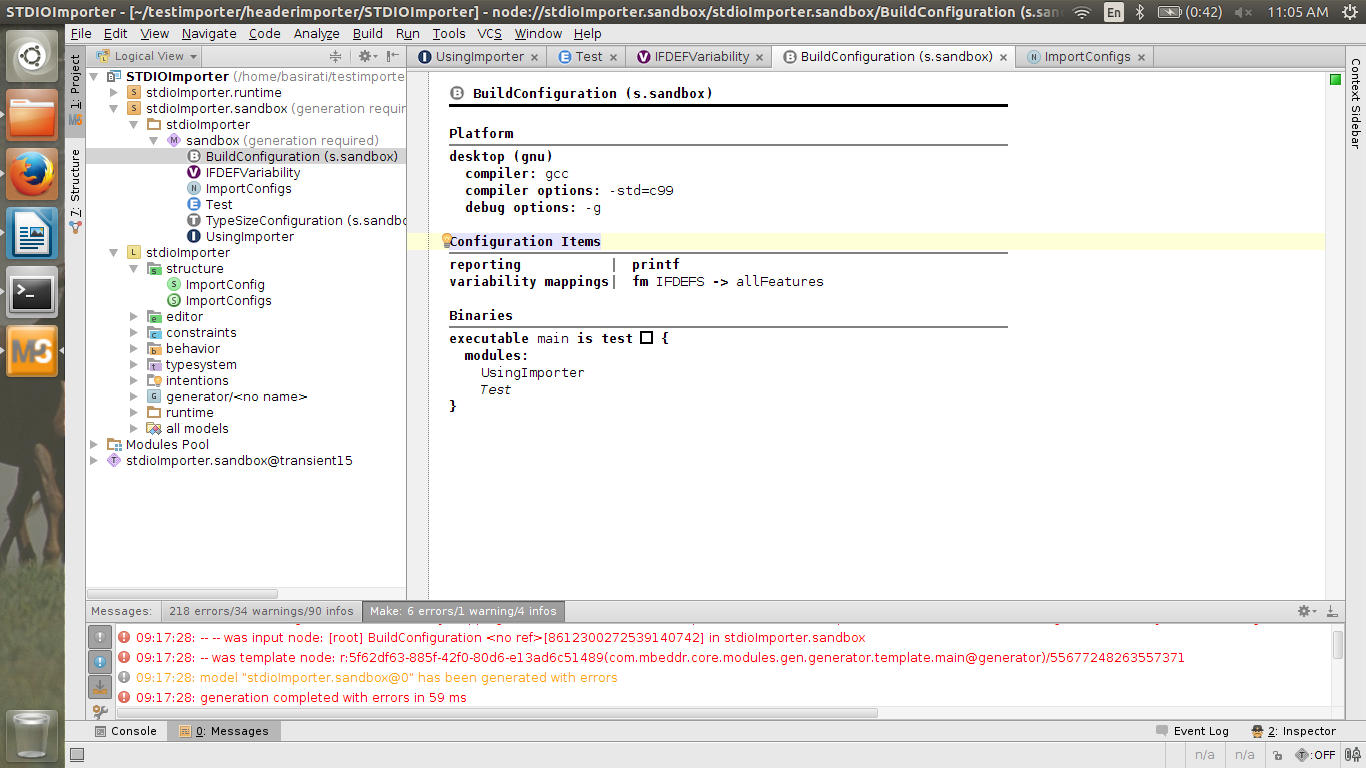
\includegraphics[scale=0.3]{buildsett.jpg}
\end{figure}

\end{itemize}



Step one and two work along in a Java project to prepare the required input for step three. The header importer tool Java project is located in folder bparser. Our scanner generator produces lexer.java file and our parser generator produces two files: sym.java and parser.java. Lexer.java will tokenize the input file. Parser.java file can recognize the tokens by their identifier which has been defined in sym.java file. The last part of the Java project consists of classes which will be used to keep header file declarations. At the last stage, MPS importer get the declarations and import them into an mbeddr external module(Figure 1).


\end{document}